\section{研究動機}
隨著時間的推移,保持健康且高效的勞動力變得愈加困難,導致該行業面臨日益嚴重的缺工問題(圖\ref{fig:example_tag})。

\begin{figure}[H]
    \centering
    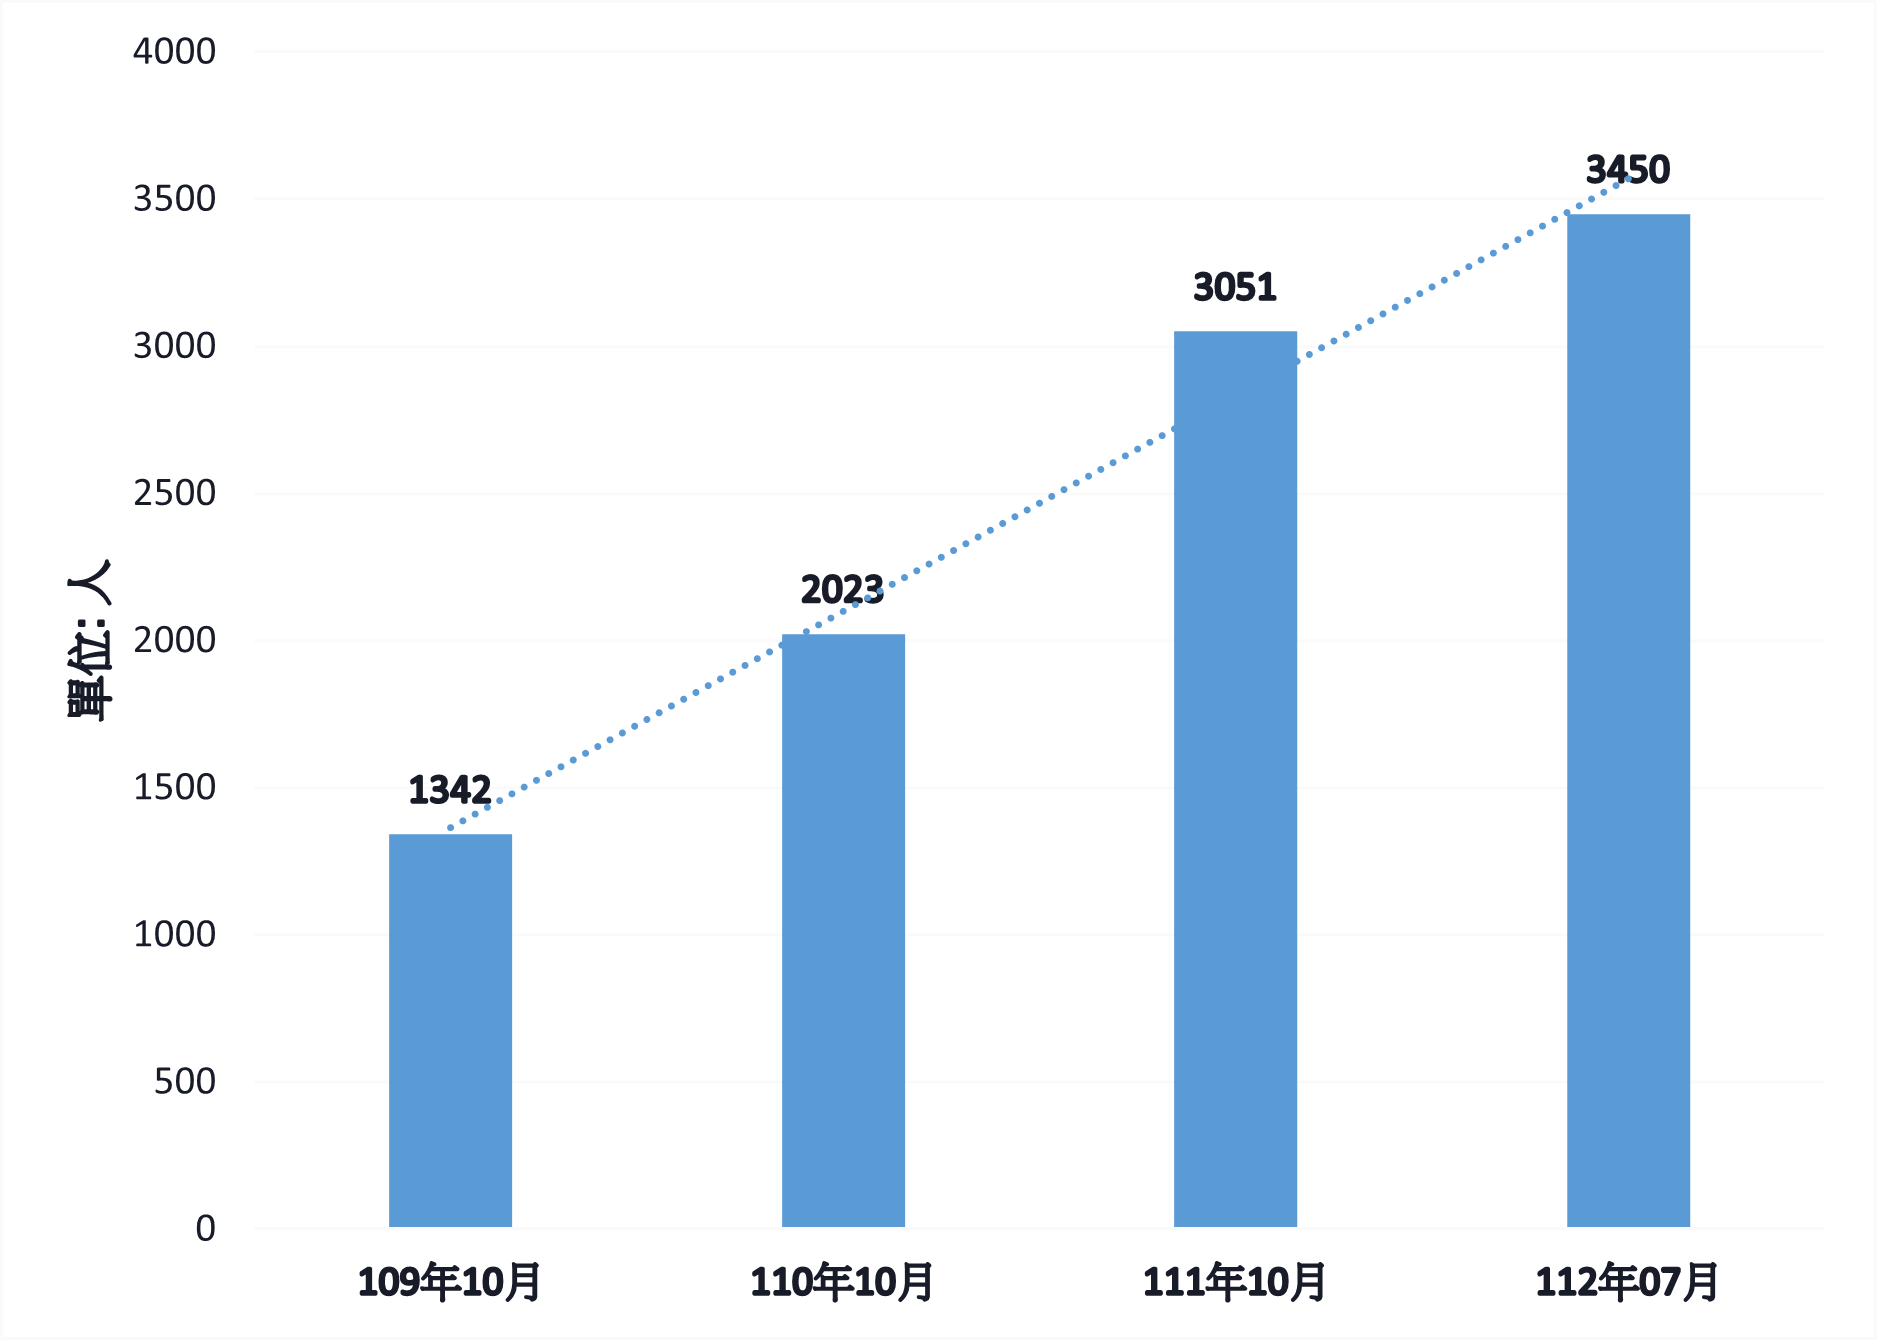
\includegraphics[width=10cm]{images/example.png}
    \caption{近四年營建工程業人力需求淨增減人數}
    \label{fig:example_tag}
\end{figure}

\section{研究目的}
解釋引入人機協作流程及數位雙生平台在建築營造行業中發展全自動化機器人的重要性,接著闡述研究目的和研究問題,並概述後續章節的內容。

\subsection{機器人於工地全自動化施作瓶頸}
解釋引入人機協作流程及數位雙生平台在建築營造行業中發展全自動化機器人的重要性,接著闡述研究目的和研究問題,並概述後續章節的內容。

\subsubsection{\Ssd{1}解析協作機器人位移規劃之資訊與操控需求} % ssd = subsubsection decoration
解釋引入人機協作流程及數位雙生平台在建築營造行業中發展全自動化機器人的重要性,接著闡述研究目的和研究問題,並概述後續章節的內容。

\subsubsection{第一章:緒論}
解釋引入人機協作流程及數位雙生平台在建築營造行業中發展全自動化機器人的重要性,接著闡述研究目的和研究問題,並概述後續章節的內容。

{\highlight 第一章:緒論}\\ % no indent and small padding in y direction
解釋引入人機協作流程及數位雙生平台在建築營造行業中發展全自動化機器人的重要性,接著闡述研究目的和研究問題,並概述後續章節的內容。

{\highlight 第一章:緒論} % have indent and small padding in y direction

解釋引入人機協作流程及數位雙生平台在建築營造行業中發展全自動化機器人的重要性,接著闡述研究目的和研究問題,並概述後續章節的內容。

\section{研究目的}

\subsubsection{\Ssd{1}解析協作機器人位移規劃之資訊與操控需求}

\subsubsection{\Ssd{2}改善建築資訊模型應用方法}

\subsubsection{\Ssd{3}建構數位雙生的人機協作平台}

\subsubsection{\Ssd{4}蒐集用於人工智慧訓練的虛實整合資料}